\section{选择一个编辑器}

haXe安装好后,其中包含了haXe的编译器、haxelib库配置工具、haxedoc文档生成工具等,但并没有包含一个合适的编辑器。因此我们还需要选择一个合适的编辑器以用来编辑haXe。在haXe的官方网站上提供了大量的常见编辑器配置文件(http://haxe.org/com/ide),可以自行选择自己喜欢的编辑器。在本书中,由于篇幅所限,不能提供所有编辑器的安装和配置介绍。在本书中,我们推荐使用开源的编辑软件Gedit。下面介绍Gedit的配置方法。

Gedit是Gnome项目的一个子项目。目前有Windows、Linux和MAC版本。Linux下Gnome环境默认即有Gedit软件,如采用KDE等桌面环境,可以自行在软件源中安装。Windows版本的下载地址如下\footnote{由于MAC下有更好的TextMate编辑器,因此请直接下载使用TextMate编辑器的语法文件,在此不再介绍MAC平台下的配置。}:

\begin{lstlisting}
`Windows版本:'
`http://ftp.gnome.org/pub/gnome/binaries/win32/gedit/'
\end{lstlisting}

请自行选择最新版本下载安装。

安装好Gedit软件后,需要该软件其进行配置方可使用。在本书的附件中tools/gedit config目录下有Gedit的haxe高亮语法文件,linux用户请将其复制到 /usr/share/gtksourceview-2.0/language-specs目录下(需要用root权限,或者在命令行中用sudo授予权限)。Windows用户请复制到Gedit安装目录下的share{\textbackslash}gtksourceview-2.0{\textbackslash}language-specs目录下。

接下来,我们把Gedit配置得更像一个IDE,以方便我们在开发中的使用。

\begin{wrapfigure}{r}{6.5cm}
\label{configedgedit}
\centering
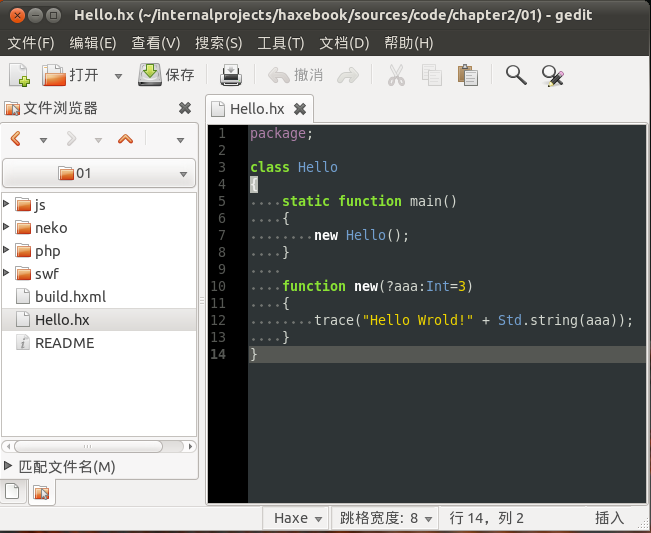
\includegraphics[width=6.5cm]{images/0001}
\caption{配置好的Gedit}
\end{wrapfigure}

选择菜单中的编辑-首选项,先打开“插件”选项卡,在插件列表中点击右键,选择“全部激活”。

接下来切换到“字体和颜色”选项卡,配色方案选择“Oblivion”。

之后切换到“编辑器”选项卡,将跳格宽度设置为8,去掉“插入空格代替制表符”的勾选;勾选“启用自动缩进”;接着取消本选项卡后面所有选项的勾选。

最后切换回“查看”选项卡,除“显示右边距”选项外,其他选项全部勾选。点击确定关闭首选项。

配置完毕后,在“查看”菜单中,勾选侧边栏选项,即完成了Gedit的配置。配置后的Gedit软件如图{\ref{configedgedit}}所示。

